%%%%%%%%%%%%%%%%%%%%%%%%%%%%%%%%%%%%%%%%%%%%%%%%%%%%%%%%%%%%%%%%%%%%%%%%%%%%%%%
% Chapter 'Refrigerants - R-152a'
%%%%%%%%%%%%%%%%%%%%%%%%%%%%%%%%%%%%%%%%%%%%%%%%%%%%%%%%%%%%%%%%%%%%%%%%%%%%%%%
\section{R-152a}
%
%%%%%%%%%%%%%%%%%%%%%%%%%%%%%%%%%%%%%%%%%%%%%%%%%%%%%%%%%%%%%%%%%%%%%%%%%%%%%%%
%%%%%%%%%%%%%%%%%%%%%%%%%%%%%%%%%%%%%%%%%%%%%%%%%%%%%%%%%%%%%%%%%%%%%%%%%%%%%%%
\subsection{Vapor Pressure - Antoine - ID 1}
%
\begin{tabular}[l]{|lp{11.5cm}|}
\hline
\addlinespace

\textbf{Name:} & R-152a \\
\textbf{Equation:} & VaporPressure\_Antoine \\
\textbf{ID:} & 1 \\
\textbf{Reference:} & P.J. Linstrom and W.G. Mallard, Eds., NIST Chemistry WebBook, NIST Standard Reference Database Number 69, National Institute of Standards and Technology, Gaithersburg MD, 20899, https://doi.org/10.18434/T4D303. \\
\textbf{Comment:} & None \\

\addlinespace
\hline
\end{tabular}
\newline

\textbf{Equation and parameters:}
\newline
%
Vapor pressure $p_\mathrm{sat}$ in $\si{\pascal}$ is calculated depending on temperature $T$ in $\si{\kelvin}$ by:
%
\begin{equation*}
\nicefrac{p_\mathrm{sat}}{100000} = 10^{a - \nicefrac{b}{T + c}}
\end{equation*}
%
The parameters of the equation are:
%
\begin{longtable}[l]{lll|lll}
\toprule
\addlinespace
\textbf{Par.} & \textbf{Unit} & \textbf{Value} &	\textbf{Par.} & \textbf{Unit} & \textbf{Value} \\
\addlinespace
\midrule
\endhead

\bottomrule
\endfoot
\bottomrule
\endlastfoot
\addlinespace

$a$ & - & 4.234060000e+00 & $c$ & $\si{\kelvin}$  & -3.471400000e+01 \\
$b$ & $\si{\kelvin}$ & 8.961710000e+02 & & & \\

\addlinespace\end{longtable}

\textbf{Validity:}
\newline
Equation is approximately valid for $160.7 \si{\kelvin} \leq T \leq 246.7 \si{\kelvin}$.
\newline

\textbf{Visualization:}
%
\begin{figure}[!htp]
{\noindent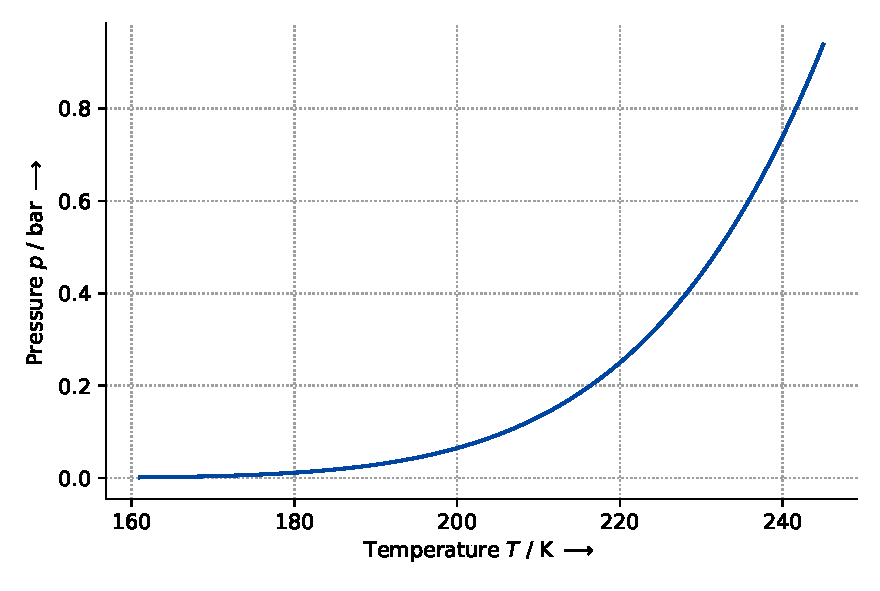
\includegraphics[height=10cm, keepaspectratio]{figs/ref/ref_R-152a_VaporPressure_Antoine_1.pdf}}
\end{figure}
%

\FloatBarrier
\newpage
%%%%%%%%%%%%%%%%%%%%%%%%%%%%%%%%%%%%%%%%%%%%%%%%%%%%%%%%%%%%%%%%%%%%%%%%%%%%%%%
%%%%%%%%%%%%%%%%%%%%%%%%%%%%%%%%%%%%%%%%%%%%%%%%%%%%%%%%%%%%%%%%%%%%%%%%%%%%%%%
\subsection{Vapor Pressure - EoSCubic - ID 1}
%
\begin{tabular}[l]{|lp{11.5cm}|}
\hline
\addlinespace

\textbf{Name:} & R-152a \\
\textbf{Equation:} & VaporPressure\_EoSCubic \\
\textbf{ID:} & 1 \\
\textbf{Reference:} & Lemmon, E. W.; Bell, I. H.; Huber, M. L.; McLinden, M. O. (2018): NIST Standard Reference Database 23. Reference Fluid Thermodynamic and Transport Properties-REFPROP, Version 10.0, National Institute of Standards and Technology. Online: https://www.nist.gov/srd/refprop. \\
\textbf{Comment:} & None \\

\addlinespace
\hline
\end{tabular}
\newline

\textbf{Equation and parameters:}
\newline
%
Vapor pressure $p_\mathrm{sat}$ in $\si{\pascal}$ is calculated depending on temperature $T$ in $\si{\kelvin}$ and molar volume v in $\si{\mole\per\cubic\meter}$ by using cubic equation of state. For this purpose, molar volumes of liquid and vapor phase are changed iteratively until fugacity coefficients of vapor and liquid phase are equal. Cubic equation of state is given by:
\begin{equation*}
\begin{split}
p &=& R \frac{T}{v - b} - \frac{a}{v \left(v + b\right)} & \quad\text{, and} \\
a &=& \frac{1}{9 \left(2^{\nicefrac{1}{3}} - 1\right)} \frac{\left(R T_\mathrm{crit} \right)^2}{p_\mathrm{crit}} \alpha & \quad\text{, and} \\
b &=& 0.08664 R \frac{T_\mathrm{crit}}{p_\mathrm{crit}} & \quad\text{, and} \\
\alpha &=& \left(1 + \kappa \left(1 - \sqrt(\nicefrac{T}{T_\mathrm{crit}}) \right) \right)^2 & \quad\text{, and} \\
\kappa &=& 0.48508 + 1.55171 \omega - 0.15613 \omega^2 & \quad\text{.}
\end{split}
\end{equation*}
%
The parameters of the equation are:
%
\begin{longtable}[l]{lll|lll}
\toprule
\addlinespace
\textbf{Par.} & \textbf{Unit} & \textbf{Value} &	\textbf{Par.} & \textbf{Unit} & \textbf{Value} \\
\addlinespace
\midrule
\endhead

\bottomrule
\endfoot
\bottomrule
\endlastfoot
\addlinespace

EoS & - & -5.000000000e+00 & $\beta_0$ & - & 0.000000000e+00 \\
$T_\mathrm{crit}$ & $\si{\kelvin}$ & 3.864100000e+02 & $\beta_1$ & - & 0.000000000e+00 \\
$p_\mathrm{crit}$ & $\si{\pascal}$ & 4.516800000e+06 & $\beta_2$ & - & 0.000000000e+00 \\
$\omega$ & - & 2.752100000e-01 & $\beta_3$ & - & 0.000000000e+00 \\
$\kappa_1$ & - & 0.000000000e+00 & & & \\

\addlinespace\end{longtable}

\textbf{Validity:}
\newline
Equation is approximately valid for $177.744 \si{\kelvin} \leq T \leq 328.4485 \si{\kelvin}$.
\newline

\textbf{Visualization:}
%
\begin{figure}[!htp]
{\noindent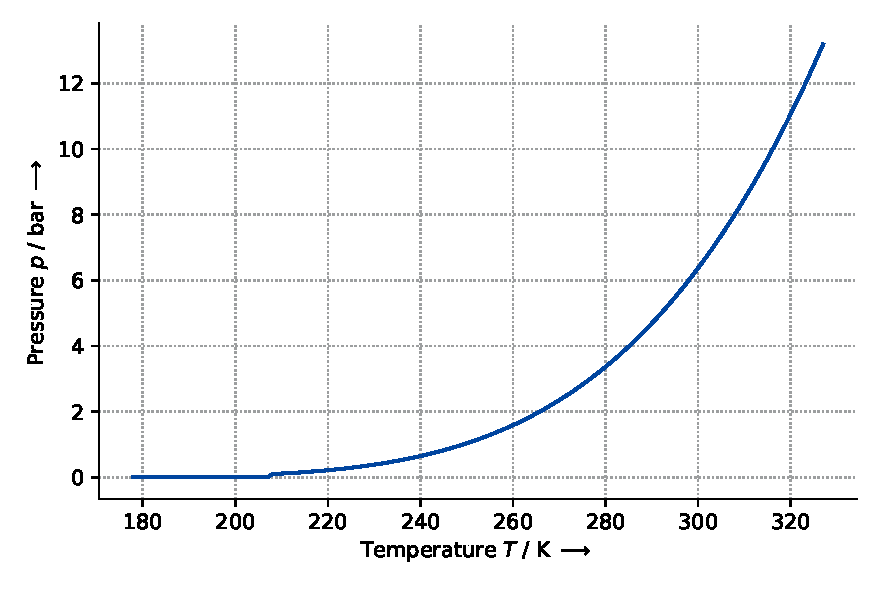
\includegraphics[height=10cm, keepaspectratio]{figs/ref/ref_R-152a_VaporPressure_EoSCubic_1.pdf}}
\end{figure}
%

\FloatBarrier
\newpage
%%%%%%%%%%%%%%%%%%%%%%%%%%%%%%%%%%%%%%%%%%%%%%%%%%%%%%%%%%%%%%%%%%%%%%%%%%%%%%%
%%%%%%%%%%%%%%%%%%%%%%%%%%%%%%%%%%%%%%%%%%%%%%%%%%%%%%%%%%%%%%%%%%%%%%%%%%%%%%%
\subsection{Vapor Pressure - EoSCubic - ID 2}
%
\begin{tabular}[l]{|lp{11.5cm}|}
\hline
\addlinespace

\textbf{Name:} & R-152a \\
\textbf{Equation:} & VaporPressure\_EoSCubic \\
\textbf{ID:} & 2 \\
\textbf{Reference:} & Lemmon, E. W.; Bell, I. H.; Huber, M. L.; McLinden, M. O. (2018): NIST Standard Reference Database 23. Reference Fluid Thermodynamic and Transport Properties-REFPROP, Version 10.0, National Institute of Standards and Technology. Online: https://www.nist.gov/srd/refprop. \\
\textbf{Comment:} & None \\

\addlinespace
\hline
\end{tabular}
\newline

\textbf{Equation and parameters:}
\newline
%
Vapor pressure $p_\mathrm{sat}$ in $\si{\pascal}$ is calculated depending on temperature $T$ in $\si{\kelvin}$ and molar volume v in $\si{\mole\per\cubic\meter}$ by using cubic equation of state. For this purpose, molar volumes of liquid and vapor phase are changed iteratively until fugacity coefficients of vapor and liquid phase are equal. Cubic equation of state is given by:
\begin{equation*}
\begin{split}
p &=& R \frac{T}{v - b} - \frac{a}{v \left(v + b\right) + b \left(v - b\right)} & \quad\text{, and} \\
a &=& 0.45724 \frac{\left(R T_\mathrm{crit} \right)^2}{p_\mathrm{crit}} \alpha & \quad\text{, and} \\
b &=& 0.07780 R \frac{T_\mathrm{crit}}{p_\mathrm{crit}} & \quad\text{, and} \\
\alpha &=& \left(1 + \kappa \left(1 - \sqrt(\nicefrac{T}{T_\mathrm{crit}}) \right) \right)^2 & \quad\text{, and} \\
\kappa &=& 0.37464 + 1.54226 \omega - 0.26992 \omega^2 & \quad\text{.}
\end{split}
\end{equation*}
%
The parameters of the equation are:
%
\begin{longtable}[l]{lll|lll}
\toprule
\addlinespace
\textbf{Par.} & \textbf{Unit} & \textbf{Value} &	\textbf{Par.} & \textbf{Unit} & \textbf{Value} \\
\addlinespace
\midrule
\endhead

\bottomrule
\endfoot
\bottomrule
\endlastfoot
\addlinespace

EoS & - & 1.000000000e+01 & $\beta_0$ & - & 0.000000000e+00 \\
$T_\mathrm{crit}$ & $\si{\kelvin}$ & 3.864100000e+02 & $\beta_1$ & - & 0.000000000e+00 \\
$p_\mathrm{crit}$ & $\si{\pascal}$ & 4.516800000e+06 & $\beta_2$ & - & 0.000000000e+00 \\
$\omega$ & - & 2.752100000e-01 & $\beta_3$ & - & 0.000000000e+00 \\
$\kappa_1$ & - & 0.000000000e+00 & & & \\

\addlinespace\end{longtable}

\textbf{Validity:}
\newline
Equation is approximately valid for $177.744 \si{\kelvin} \leq T \leq 328.4485 \si{\kelvin}$.
\newline

\textbf{Visualization:}
%
\begin{figure}[!htp]
{\noindent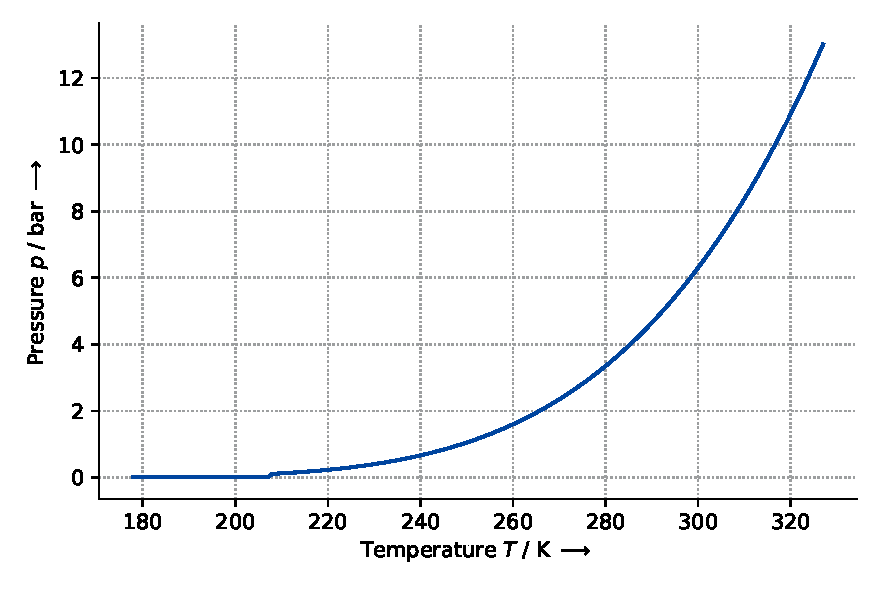
\includegraphics[height=10cm, keepaspectratio]{figs/ref/ref_R-152a_VaporPressure_EoSCubic_2.pdf}}
\end{figure}
%

\FloatBarrier
\newpage
%%%%%%%%%%%%%%%%%%%%%%%%%%%%%%%%%%%%%%%%%%%%%%%%%%%%%%%%%%%%%%%%%%%%%%%%%%%%%%%
